\documentclass[review]{elsarticle} %review=doublespace preprint=single 5p=2 column
%%% Begin My package additions %%%%%%%%%%%%%%%%%%%

\makeatletter
\def\ps@pprintTitle{%
 \let\@oddhead\@empty
 \let\@evenhead\@empty
 \def\@oddfoot{\it \hfill\today}%
 \let\@evenfoot\@oddfoot}
\makeatother

% A modified page layout
\textwidth 6.75in
\oddsidemargin -0.15in
\evensidemargin -0.15in
\textheight 9in
\topmargin -0.5in
%%%%%%%%%%%%%%%% end my additions to header


\usepackage{amssymb,amsmath}
\usepackage{hyperref}

\begin{document}
\begin{frontmatter}
  \title{No indicators for stochastic transitions but establishing baselines for
         early warning signals remains a general challenge}
  \author[cstar]{Carl Boettiger\corref{cor1}}
  \cortext[cor1]{Corresponding author}
  \ead{cboettig@ucsc.edu}
  \address[cstar]{Center for Stock Assessment Research, Department of Applied Math and Statistics, University of California, Mail Stop SOE-2, Santa Cruz, CA 95064, USA}
  \author[esp]{Alan Hastings}
  \address[esp]{Department of Environmental Science and Policy, University of California, Davis, CA, 95616 United States}
 \end{frontmatter}


In Boettiger \& Hastings {[}1{]} we demonstrated that conditioning on
observing a purely stochastic transition from one stable basin to
another could generate time-series trajectories that could be mistaken
for an early warning signal of a critical transition (such as might be
due to a fold bifurcation; {[}2{]}, when instead the shift is merely due
to chance. While the goal was to highlight a potential danger in mining
historical records for patterns showing sudden shifts when seeking to
test early warning techniques, Drake {[}3{]} draws attention to a
potentially more interesting consequence of our analysis. Drake argues
that the bias observed could be used to forecast purely stochastic
transitions -- a task previously thought to be impossible {[}4{]}.
Unfortunately, we feel this interpretation too generous and must agree
with the prevailing opinion that early warning signals for purely
stochastic transitions do not exist. Drake demonstrates how the patterns
presented in {[}1{]} show an indisputable difference between the time
series that transition by chance and the much larger population of
replicate time series driven by the identical mechanism that do not
transition by chance. We argue that the appropriate null distribution is
the subset of trajectories that had experienced an equally large
deviation. Both numerical and analytical work show that the apparent
signal to which Drake refers is an artifact of a large deviation, rather
than than the probability of an impending transition.

What is meant by having found evidence of an early warning signal? We
can only define this relative to some null distribution or baseline
indicating what we might expect when no warning signal is present. This
question has so far received insufficient attention, empirical and
theoretical, throughout the recent literature on the subject {[}5{]}.
Drake's analysis presents the choice of baseline or null distribution as
the population of all replicates experiencing the identical dynamics. We
argue that the appropriate null distribution in this case would rather
be only the subset of those trajectories that had experienced an equally
large deviation (with or without experiencing a transition), rather than
the entire population. After all, our goal is to detect approaching
transitions before they happen, not merely detect large deviations after
they happen.

A numerical example shows that a similar pattern to that observed
{[}1{]} can be seen in the large deviations of a purely stable system.
This suggests that the pattern is not due to the curvature or any other
feature of the chance transition, but only due to the conditional
selection being biased to such chance transitions. We also discuss some
earlier analytic work which helps explain the patterns observed.

We replicate the analysis of Boettiger and Hastings {[}1{]} using time
series replicates produced by an Ornstein-Uhlenbeck (OU) process: a
stochastic differential equation in which there is only a single optimum
whose strength is proportional to the displacement,

\[ dX = - \alpha X dt + \sigma dBt \]

Instead of conditioning on trajectories that experience a large
deviation, we condition on trajectories that experience a very large
deviation. We then compute warning signals for each of these large
deviation trajectories, and compare their distribution to that of the
entire population of trajectories as shown in Figure 1. We note that the
same bias is observed. This should help illustrate that observations we
reported are driven by the large deviation preceding the transition, and
are simply evidence of this fact and not of an impending transition per
se. While trajectories already far from the origin are more likely to
transition than ones close to the average, such events can be trivially
identified by comparing their states to the historical average.

\begin{figure}[htbp]
\centering
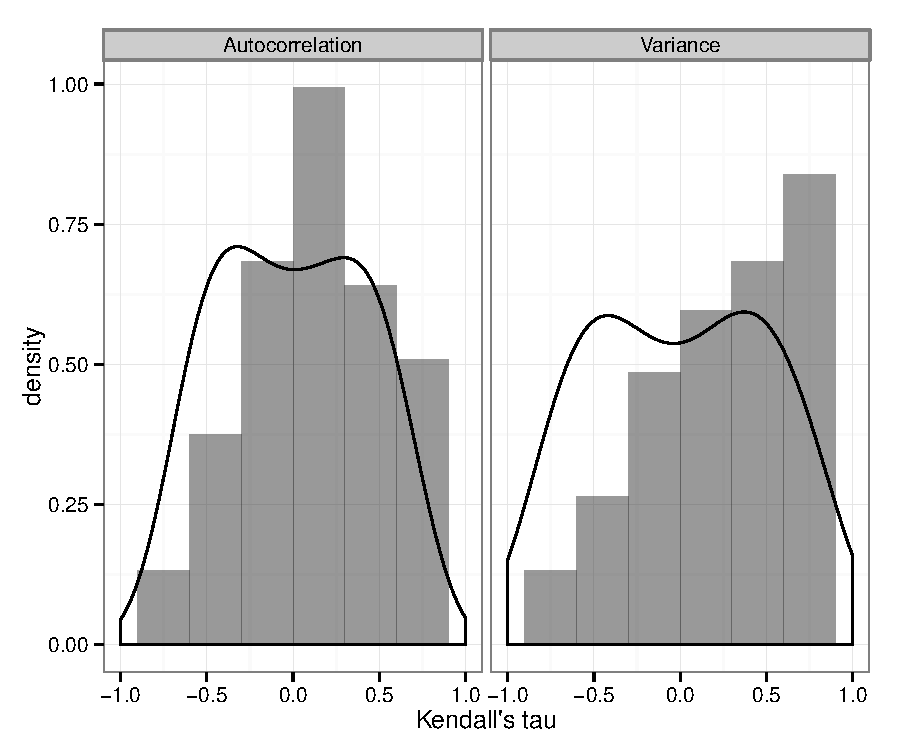
\includegraphics{figure1.eps}
\caption{Figure 1. Histogram shows the frequency the correlation
statistic $\tau$ observed for each warning signal (variance,
autocorrelation coefficient) on the large deviation samples. Background
distribution of all samples show by smooth line (kernel density
estimate). More positive values of tau are supposed to indicate a rising
indicator which can be a signal of an approaching transition {[}2{]}.
$\alpha = 5$, $\sigma=3.5$, $t \in (0, 10)$, 2000 replicates, 20,000
sample points each. Conditionally selected trajectories experiencing a
deviation of at least -4, and analyzed the 1,500 data points prior to
the threshold to determine a warning signal (following Reference 6).
(\href{https://raw.github.com/cboettig/earlywarning/7460ea94c293844d8e88c83b95e3d80004817de6/inst/examples/beer.md}{link to code},
\href{https://raw.github.com/cboettig/earlywarning/7460ea94c293844d8e88c83b95e3d80004817de6/inst/examples/beer_nulldat.csv}{null distribution data},
\href{https://raw.github.com/cboettig/earlywarning/7460ea94c293844d8e88c83b95e3d80004817de6/inst/examples/beer_dat.csv}{conditional distribution data})}
\end{figure}

Observing the bias shown in Figure 1 depends on having a rapid enough
sample frequency to capture the escape trajectory and a long enough
trajectory for the statistic to demonstrate an increase over time. Since
large deviations due to stochastic forces alone must be fast so must the
accompanying warning signal and managemnt response, which will show up
on the time scale of the perturbation. Of course fast relative to the
system dynamics, may or may not be fast relative to the timescale of
management; just as in the case of bifurcation-driven warning signals,
see Reference 7.

The realization that the trajectories of large deviations have a pattern
that looks like an early warning signal can be better understood in
light of early work on large deviations. Reference 1 observes that any
trajectory that does manage to escape by chance does so quickly. This
rapid dash to the boundary results in an escape path that is highly
autocorrelated and marked by a rapid increase in variance as it departs
from the mean. It turns out that we can be more precise about the speed
of this trajectory: the expected transit time from the vicinity of the
stable point to some distant deviation $L$ can be shown to scale as
$\log(L/\sigma)$. This result is rather remarkable considering it is the
very same scaling to go against the gradient, uphill, as the expected
time to \emph{return} downhill from that distant point $L$ to the
neighborhood of the stable point. For comparison, the waiting time to
observe such a trajectory scales as $\exp(L^2/\sigma^2)$, such that we
must wait a long time before observing such a path. These results follow
in the limit of $L \gg \epsilon$ for a region $\epsilon$ around the
stable point and for small noise $\sigma \ll L$, and a careful walk
through of the calculation can be found in Reference 8 for the OU
process as considered here, which follows the derivation of Reference 9.
This result has been rediscovered in other ecological and evolutionary
contexts, e.g. Reference 10, and Drake and Griffen in fact provide an
impressive empirical demonstration of the phenomenon in recovery and
extinction patterns in Reference 11. It is a direct consequence of this
rapid trajectory that the resulting pattern shows a sudden rise in
variance and autocorrelation as the random walk follows its trajectory
to the large deviation. More precise statements for the expected
variance and autocorrelation along such a trajectory could be solved for
along these same lines (or more directly through the large deviation
theory, see Reference 12) but are beyond the scope of this comment.

Both the numerical and analytic lines of evidence suggest that pattern
Drake alludes arises from the large deviation, rather than from some
signal that the system approaches a stochastic transition per se. If we
are to consider this a warning signal of stochastic transitions, it is
only in this weak sense in which the signal can be seen in any large
deviation rather than being sufficient evidence of the chance
transition. Relative to the background of all trajectories obeying the
same dynamics, this has positive predictive value. Relative only to
other large deviations, it does not. We heartily agree with the need for
a decision-theoretic approach to early warning signal questions
{[}13{]}. The challenge of sufficient or unique early warning indicators
is not limited to stochastic shifts, but includes the more typical
critical transitions. For instance, rising variance or autocorrelation
patterns typical of fold bifurcations can be observed in more benign
bifurcations or smooth transitions {[}14{]}. Early warning signals may
offer a promising technique that will one day allow us to avoid
seemingly unpredictable catastrophes -- but we must not lose sight of
just how difficult are the challenges involved. A key step here and for
early warning indicators more generally is to understand these other
circumstances in which they can arise, that we may then develop ways to
eliminate those possibilities. Though we may never be able to detect
purely stochastic transitions, perhaps these approaches in this
discussion may lead to more unique and sufficient indicators for true
critical transitions.

1 Boettiger, C. \& Hastings, A. 2012 Early warning signals and the
prosecutor's fallacy. \emph{Proceedings of the Royal Society B:
Biological Sciences} (doi:10.1098/rspb.2012.2085)

2 Scheffer, M. et al. 2009 Early-warning signals for critical
transitions. \emph{Nature} \textbf{461}, 53--9.

3 Drake, J. M. 2013 Early warning signals of stochastic switching.
\emph{Proceedings of The Royal Society B} \textbf{in press}.

4 Lenton, T. M. 2011 Early warning of climate tipping points.
\emph{Nature Climate Change} \textbf{1}, 201--209.
(doi:10.1038/nclimate1143)

5 Boettiger, C. \& Hastings, A. 2013 Tipping points: From patterns to
predictions. \emph{Nature} \textbf{493}, 157--158. (doi:10.1038/493157a)

6 Dakos, V., Scheffer, M., van Nes, E. H., Brovkin, V., Petoukhov, V. \&
Held, H. 2008 Slowing down as an early warning signal for abrupt climate
change. \emph{Proceedings of the National Academy of Sciences}
\textbf{105}, 14308--12. (doi:10.1073/pnas.0802430105)

7 Hughes, T. P., Linares, C., Dakos, V., van de Leemput, I. a \& van
Nes, E. H. 2013 Living dangerously on borrowed time during slow,
unrecognized regime shifts. \emph{Trends in ecology \& evolution}
\textbf{28}, 149--55. (doi:10.1016/j.tree.2012.08.022)

8 Mangel, M. 2006 \emph{The Theoretical Biologist's Toolbox:
Quantitative Methods for Ecology and Evolutionary Biology}. Cambridge
University Press.

9 Ludwig, D. 1981 Escape from Domains of Attraction for Sytstems
Perturbed by Noise. In \emph{Nonlinear Phenomena in Physics and Biology}
(eds R. H. Enns B. L. Jones R. M. Miura \& S. S. Rangnekar), pp.
549--566. Boston, MA: Springer New York.

10 Lande, R. 1985 Expected time for random genetic drift of a population
between stable phenotypic states. \emph{Proceedings of the National
Academy of Sciences} \textbf{82}, 7641--7645.

11 Drake, J. M. \& Griffen, B. D. 2009 Speed of expansion and extinction
in experimental populations. \emph{Ecology letters} \textbf{12}, 772--8.
(doi:10.1111/j.1461-0248.2009.01325.x)

12 Freidlin, M. I., Wentzell, A. D., Freidlin, M. I. \& Wentzell, A. D.
1998 \emph{Random Perturbations of Dynamical Systems (Grundlehren der
mathematischen Wissenschaften)}. Springer.

13 Boettiger, C. \& Hastings, A. 2012 Quantifying limits to detection of
early warning for critical transitions. \emph{Journal of The Royal
Society Interface} \textbf{9}, 2527--2539. (doi:10.1098/rsif.2012.0125)

14 Kéfi, S., Dakos, V., Scheffer, M., Van Nes, E. H. \& Rietkerk, M.
2012 Early warning signals also precede non-catastrophic transitions.
\emph{Oikos} (doi:10.1111/j.1600-0706.2012.20838.x)

\end{document}


